\documentclass{amsart}[12pt]
\usepackage{amsmath, amsfonts, tikz, natbib, array, textcomp}
\oddsidemargin=0in \evensidemargin=0in
\textwidth=6.6in \textheight=8.7in

\title{A variation on the Chamberlin Trimetric map projection}
\author{B R S Recht}
\date{January 2020}

\begin{document}

\begin{abstract}
   A variation of the Chamberlin Trimetric map projection is presented. This
   projection amounts to a linear transformation of the squares of the distances
   from a given point to three control points. It is significantly simpler to
   calculate than the Chamberlin projection, and allows for an inverse
   projection in the spherical approximation which only requires numerical
   estimation of one parameter. While it introduces slightly more distortion,
   the difference is small enough to be unnoticeable in most common use cases.
\end{abstract}
\maketitle

\section{Introduction}
A map projection is a projection from a sphere or an ellipsoid -- such as one
being used to model the surface of the earth -- to the plane. Map projections
that preserve angles are called conformal; ones that preserve the relative area
of shapes may be termed authalic, equal-area, equiareal or equivalent. All map
projections introduce some form of distortion: no map projection may be both
conformal and authalic.\cite{snyder87} A compromise map projection is one that
is neither conformal nor authalic, but seeks to balance different kinds of
distortion.

The Chamberlin Trimetric projection is a compromise map projection that achieves
a balance between distortions in area, angle, and distance. The National
Geographic Society has published wall and atlas maps using this projection. In
contrast to most projections, which are analytically specified, the Chamberlin
projection has a simple geometric construction. Three control points on the
globe are specified, and a triangle in the plane is constructed having the same
distances between its vertices as the true distances between the points on the
globe. True distances from those control points to a given point on the globe
are measured, and arcs are drawn at those distances from their respective
points in the plane. The arcs form a small triangle: a point in that triangle
is chosen as the projection of the original point.\cite{christensen}
Originally, in the 1950s when manual plotters were used, the exact definition
of this point was not important, but \cite{christensen} and most modern
implementations (e.g. \cite{proj}) use the centroid of the triangle formed by
the points where each pair of circles intersect. Thus, the Chamberlin
projection is a form of triangulation: it is also a cousin of the
two-point equidistant projection.\cite{snyder89}

The geometric nature of this construction result in a somewhat involved
algorithmic form. As commented on in \cite{christensen}, there are special
cases to handle when the given point lies at a control point, or on an edge of
the triangle with vertices at the control points. This also makes analysis of
the projection somewhat more difficult, although numerical approximation of the
distortion can be performed.

In this text, we demonstrate that a slightly more complicated geometric
construction results in a map projection that is very similar to the
Chamberlin Trimetric projection but has a much simpler formula. Since the
projection is a linear function of the square of the distances from the given
point to the control points, we call it the Linear Trimetric projection. While
the Linear Trimetric introduces slightly more distortion, the difference is
small and difficult to notice by eye.

\section{Derivation of forward projection}
This derivation will make heavy use of basic linear algebra: refer to a basic
text on linear algebra, such as \cite{strang80}, if anything is
unfamiliar.

Let $\mathbf v$ be a point on some ellipsoid, and let $\mathbf p = [x, y]$
be a point in the Euclidean plane. Let $d(\mathbf v_a, \mathbf v_b)$ be the
geodesic distance between the points $\mathbf v_a$ and $\mathbf v_b$ on that
ellipsoid. Let $\|\mathbf p\| = \sqrt{x^2 + y^2}$ be the Euclidean norm of the point
$\mathbf p$, such that $\|\mathbf p_a - \mathbf p_b\|$
is the Euclidean distance between the points $\mathbf p_a$ and $\mathbf p_b$.

Let $\mathbf v_1$, $\mathbf v_2$, $\mathbf v_3$ be control points on the sphere,
and $\mathbf p_1 = [x_1, y_1]$ etc. be the image of those control points on the
plane, such that $d(\mathbf v_i, \mathbf v_j) = \|\mathbf p_i - \mathbf p_j\|$
for all $i$ and $j$ in ${1, 2, 3}$. The triangles with vertices at $\mathbf v_i$
or $\mathbf p_i$ will be called the control triangles (spherical or planar
control triangle, respectively, if the distinction is important). Without loss
of generality, also assume that $\|\mathbf p_i\|$ is the same for all $i$, such
that the center of the circumcircle of the control triangle lies at the origin.
(This just removes a translation in the plane in order to simplify the formula;
false northing and easting can be added later.)

Let $r_i = d(\mathbf v_i, \mathbf v)$ be the geodesic distance from
$\mathbf v_i$ to $\mathbf v$, but also the radius of a circle that is centered
at $\mathbf v_i$ and $\mathbf v$ lies on its boundary. The Chamberlin
projection draws a circle of radius $r_i$ around each point $\mathbf p_i$,
forming a small triangle with circular arcs for edges, and chooses a point
$\mathbf p$ as the centroid of that small triangle. Of course, each pair of
circles intersects in (at most) two places, so the implementation must take
care to choose the point of intersection that lies on the small triangle and
not the other one.

\begin{figure}%[!htbp]
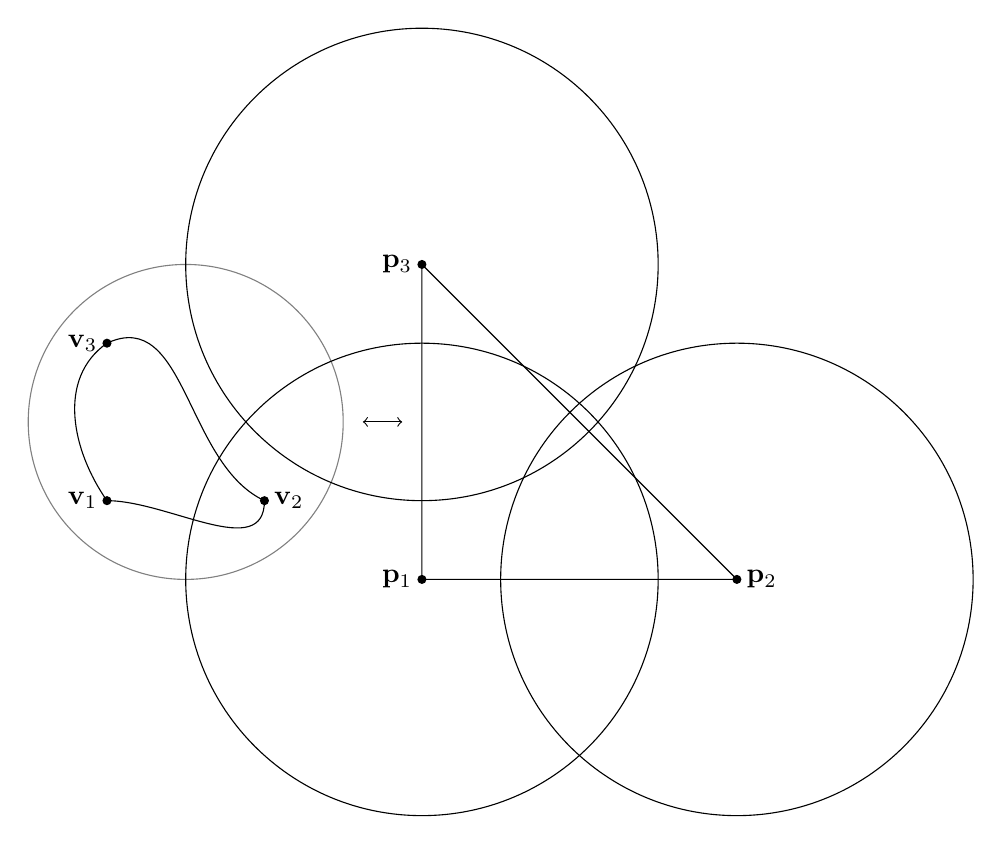
\begin{tikzpicture}
  \draw [gray] (2,2) circle [radius=2];
  \draw (1, 1) to [out=0, in=-90]
  (3, 1) to [out=155, in=25]
  (1, 3) to [out=215, in=125]
  (1, 1);
  \draw[fill] (1,1) circle [radius=0.05] node[anchor=east] {$\mathbf v_1$};
  \draw[fill] (3,1) circle [radius=0.05] node[anchor=west] {$\mathbf v_2$};
  \draw[fill] (1,3) circle [radius=0.05] node[anchor=east] {$\mathbf v_3$};

  \draw [<->] (4.25,2) -- (4.75,2);
  \draw (5, 0) -- (9, 0) -- (5, 4) -- (5, 0);
  \draw[fill] (5,0) circle [radius=0.05] node[anchor=east] {$\mathbf p_1$};
  \draw[fill] (9,0) circle [radius=0.05] node[anchor=west] {$\mathbf p_2$};
  \draw[fill] (5,4) circle [radius=0.05] node[anchor=east] {$\mathbf p_3$};
  \draw (5,0) circle [radius=3];
  \draw (9,0) circle [radius=3];
  \draw (5,4) circle [radius=3];

\end{tikzpicture}
\caption{Depiction of Chamberlin projection.}
\label{fig:chamberlin}
\end{figure}

One can make two observations on this configuration of circles in the plane. One
is that the two points of intersection of each pair of circles are symmetric
about the triangle edge between the two control points. The other is that, if
one draws a line through the two points of intersection of each pair of circles,
that line is perpendicular to the triangle edge, and once the lines are drawn
for each pair of circles, the three lines appear to meet at the same point.
(That observation will be proven true momentarily.) Although that point is not
necessarily within the small triangle, it is for most points within the control
triangle.

Suppose that $\mathbf p_1 = [-1,0]$ and $\mathbf p_2 = [1,0]$. Then the points
of intersection of the circles with radius $r_1$ and $r_2$ are given as so:
\begin{equation}\begin{split}
x =& \frac{r^2_1 - r^2_2}{4}\\
y =& \pm \frac{1}{4} \sqrt{-
\left(r_1 - r_2 - 2\right)
\left(r_1 - r_2 + 2\right)
\left(r_1 + r_2 - 2\right)
\left(r_1 + r_2 + 2\right)}
\end{split}\end{equation}
Note that there is not necessarily a real solution for $y$. In that case, the
circles do not intersect.

If a line passing through the two points of intersection is drawn, it intersects
the triangle edge from $\mathbf p_1$ to $\mathbf p_2$ perpendicularly at
the point with $x$ as above and $y=0$: call that point $\mathbf p_{12}$. In
general form, one can use linear interpolation to determine the point of
perpendicular intersection $\mathbf p_{ij}$ as so:
\begin{equation}\label{eq:pij}
\mathbf p_{ij} = \mathbf p_i \frac{1-t_{ij}}{2} + \mathbf p_j \frac{1+t_{ij}}{2}
\end{equation}
\begin{equation}
t_{ij} = \frac{r_i^2 - r_j^2}{\| \mathbf p_i - \mathbf p_j \|^2}
\end{equation}
Note that this is defined for all $r_i$, regardless of whether the circles
intersect.

The lines passing through $\mathbf p_{ij}$ and parallel to the line from
$p_i$ to $p_j$ all meet at the same point. This can be proven with a simple
triangle theorem sometimes attributed to Carnot: such lines meet at a single
point if and only if \cite{posamentier}\cite{wohlgemuth}
\begin{equation}
  \|\mathbf p_1 - \mathbf p_{12}\| +
  \|\mathbf p_2 - \mathbf p_{23}\| +
  \|\mathbf p_3 - \mathbf p_{31}\| =
  \|\mathbf p_2 - \mathbf p_{12}\| +
  \|\mathbf p_3 - \mathbf p_{23}\| +
  \|\mathbf p_1 - \mathbf p_{31}\|
\end{equation}
for points $\mathbf p_{ij}$ lying on the edge between $\mathbf p_i$ and
$\mathbf p_j$. Plugging in Equation \ref{eq:pij} and simplifying proves that
these lines satisfy this theorem.

The equation of the line passing from $\mathbf p_i$ to $\mathbf p_j$ is:
\begin{equation}
y (x_i - x_j) - x (y_i - y_j) - x_i y_j - x_j y_i = 0.
\end{equation}
Thus, the equation of the line perpendicular to that line and passing through
the point $\mathbf p_{ij}$ can be found to be
\begin{equation}
y (y_i - y_j) + x (x_i - x_j) + \frac{r_i^2 - r_j^2}{2} = 0.
\end{equation}
Combining the equation of each perpendicular line creates a linear system.
It is an overdetermined system of 3 equations in 2 variables, but since all 3
perpendicular lines meet at the same point as proven above, it has a solution.
Ultimately this system can be solved for $\mathbf p$ to define a map projection
as follows. Let $\mathbf P$ be a 3x2 matrix having $\mathbf p_i$ as its $i$th
column. Then:
\begin{equation}\label{eq:forward}
\mathbf p = \mathbf M \begin{bmatrix} r^2_1 & r^2_2 & r^2_3 \end{bmatrix}^\top,
\end{equation}
\begin{equation}
\mathbf M = \frac{1}{2T}
\begin{bmatrix} y_3 - y_2 & y_1 - y_3 & y_2 - y_1 \\
x_2 - x_3 & x_3 - x_1 & x_1 - x_2 \end{bmatrix} = \frac{1}{2T}
\begin{bmatrix} 0 & -1  \\
1 & 0 \end{bmatrix}
\mathbf P
\begin{bmatrix} 0 & -1 & 1 \\
1 & 0 & -1 \\
-1 & 1 & 0 \end{bmatrix},
\end{equation}
\begin{equation}
T = \begin{vmatrix} x_1 & x_2 & x_3 \\
 y_1 & y_2 & y_3 \\
 1 & 1 & 1
\end{vmatrix}.
\end{equation}
$T$ is equal to twice the area of the Euclidean control triangle. $T$ is zero
if all the control points lie on a line, and is very small if the control
points are very close to each other, in which case the matrix $\mathbf M$ is
undefined or numerically unstable.
(Of course, those are not typical use cases for the Chamberlin projection.)

The matrix $\mathbf M$ has a (right) nullspace spanned by the vector $[1,1,1]$.
In general, this implies this projection is not one-to-one for all possible
values of $r_i$: in particular, if $r_1 = r_2 = r_3$, then $\mathbf p = [0,0]$.
Of course, not all values of $r_i$ correspond to actual points on the ellipsoid,
but this projection will be observed later on to have overlap for some points
outside the control triangle, much like the Chamberlin projection.
(Again, the Chamberlin projection is not commonly used to project the entire
earth, except for demonstration purposes.)

\section{Inverse}
Given $\mathbf p$, we start to invert the projection as so:
\begin{equation}\label{eq:inverse}
\begin{bmatrix} k_1 & k_2 & k_3

\end{bmatrix}^\top = \mathbf M^+ \mathbf p,
\end{equation}
\begin{equation}
\mathbf M^+ = \frac{2}{3}
\begin{bmatrix} 2x_1 - x_2 - x_3 & 2y_1 - y_2 - y_3 \\
-x_1 + 2x_2 - x_3 & -y_1 + 2y_2 - y_3 \\
-x_1 - x_2 + 2x_3 & -y_1 - y_2 + 2y_3
\end{bmatrix} = \frac{2}{3}
\begin{bmatrix} -2 & 1 & 1 \\
1 & -2 & 1 \\
1 & 1 & -2
\end{bmatrix}
\mathbf P^\top
\end{equation}
$k_i = r^2_i - h$ for some value $h$. This is a general solution to inverting
Equation \ref{eq:forward}, thus the free parameter $h$. $\mathbf M^+$ is the
pseudoinverse of $\mathbf M$ and vice versa. Because $\mathbf M^+$ has a left
nullspace spanned by the vector $[1,1,1]$, it follows that $\sum_i k_i = 0$,
which can be used to calculate $k_i$ more efficiently.

By plugging Equation \ref{eq:forward} into Equation \ref{eq:inverse}, we can
find that $h = \frac{1}{3}\sum_i r^2_i$. Unfortunately, if one attempts to
solve for $r_i$ given $k_i$, they find another general solution with one free
parameter, putting them right back where they started. It turns out that
information about the geoid needs to be introduced to determine $r_i$ and
$\mathbf v$. In the following, this is done with spherical approximation, and
the case of an ellipsoid is discussed.

\subsection{With spherical approximation}
If treating the earth as a unit sphere, then let $\mathbf v = [x, y, z]$ be a
Euclidean vector such that its norm is 1:
$\|\mathbf v \|= \sqrt{x^2 + y^2 + z^2} = 1$.
In that case, spherical geometry allows an analytic way to determine a vector
$\mathbf v$ given $r_i$. For this section, let $r_i$ have units of radians of
arc on the surface of the sphere. The circle of points $\mathbf v$ at distance
$r_0$ from a point $\mathbf v_0$ is simply the circle where a plane intersects
the sphere. This plane may be specified as so:
\begin{equation}
  \mathbf v_0 \cdot \mathbf v = \cos\left(r_0\right).
\end{equation}
Clearly, replacing $\mathbf v_0$ with $\mathbf v_i$ and $r_0$ with $r_i$ for
each $i$ gives a linear system. Let $\mathbf V$ be the matrix having
$\mathbf v_i$ as its $i$th column. Thus,
\begin{equation}
  \mathbf v = \mathbf V^{-1} \begin{bmatrix} \cos\left(r_1\right) \\
  \cos\left(r_2\right) \\
  \cos\left(r_3\right)
  \end{bmatrix}
\end{equation}
$\mathbf V^{-1}$ is undefined or numerically ill-behaved if the control points
lie on a line or are very close together. It is also undefined if the points all
lie on a great circle of the sphere: in that case, there are two points that
satisfy the values of $r_i$. Again, those are not typical use cases for
the Chamberlin projection.

For the point to lie on the unit sphere, $\|\mathbf v\| = 1$. Let $\mathbf c$
be a vector with $i$th component $\cos\left(r_i \right)$. Then,
\begin{equation}
  \mathbf c^\top \left(\mathbf V^\top \mathbf V\right )^{-1} \mathbf c = 1
\end{equation}
Make the substitution $r_i = \sqrt{k_i + h}$. The result is a little opaque,
but we now have an equation with one unknown, $h$. Some obvious bounds can be
placed on $h$. In units of radians, $0 \le r_i \le \pi$. Since this must hold
for every $r_i$, it follows that
$$
h_{\min} = -\min_i k_i \le h \le \pi^2 - \max_i k_i = h_{\max}
$$.
Within these bounds, there may be at most two solutions for $h$. In most
applications, the solution with smaller $h$, nearer to the control triangle, is
the desirable one. Let
$\mathbf A = \left(\mathbf V^\top \mathbf V\right )^{-1}$,
where $\mathbf A$ is symmetric and positive semi-definite, and
$f(h) = \mathbf c^\top \mathbf A \mathbf c - 1$. See Figure \ref{fig:fh} for a
plot of $f(h)$ for various points.
The derivative of $f(h)$ is
\begin{equation}
  f'(h) = -\mathbf c^\top \mathbf A \mathbf b
\end{equation}
where $\mathbf b$ is the vector with $i$th component
$\mathrm{sinc}\left(\sqrt{k_i + h}\right)$, and the function $\mathrm{sinc} (x)$
is defined as so:
\begin{equation}
\mathrm{sinc} (x) = \begin{cases}
      1 & \text{if}\ x=0, \\
      \frac{\sin x}{x} & \text{otherwise}.
    \end{cases}
\end{equation}
Note that $f'(h)$ and $f(h)$ share many of the same terms, making the
calculation more efficient. If needed for numerical purposes, the compositions
of trig functions with square root can be smoothly extended to negative values:
when $x<0$, $\cos \sqrt{x} = \cosh \sqrt{-x}$
and $\frac{\sin \sqrt{x}}{\sqrt{x}} = \frac{\sinh \sqrt{-x}}{\sqrt{-x}}$.

\begin{figure}%[!htbp]

\caption{Plot of $f(h)$ for a number of points.}
\label{fig:fh}
\end{figure}

Given all the preceding, Newton's method can be applied to solve for $h$.
Using $h_{\min}$ as an initial guess, a good approximation is achieved for
points inside the control triangle within only a few iterations. Better initial
guesses are possible, but don't appear to be worth the cost of calculation.
Convergence is somewhat slower further away from the control triangle, and is
worst at the boundary of the projection. This is expected: at the boundary, the
function reaches a minimum at the same place as its root, $f(h)=f'(h)=0$, and
Newton's method converges at a merely linear rate.\cite{burden}

\subsection{Without spherical approximation}
The method for spheres is not extensible to ellipsoids. Geodesic
circles cannot in general be described as the intersection of a plane and a
surface. Also, we can no longer make the assumption that the Euclidean norm
$\|\mathbf v\|$ is constant. In general, these sort of problems are harder on
an ellipsoid than a sphere. Geodesic circles are usually calculated in most
software by brute force: extending a number of lines from a center point and
using the endpoints as an approximation of the circle.\cite{idfk}
It is not surprising that an analytic form,
or form with an easy numerical iteration, is not available here.

The spherical approximation is reasonably close to an ellipsoidal
calculation. Figure \ref{fig:roundtrip} demonstrates the results of performing
the forward transformation with the ellipsoid and then transforming it back
using the spherical inverse transformation, and then calculating the deviation
in distance of each point. Within the control triangle, the
deviation does not exceed 25 kilometers, and within the hemisphere containing the
control triangle, no more than 60 near the south pole.

\begin{figure}%[!htbp]

\caption{Deviation after round-trip transformation. Units are kilometers.}
\label{fig:roundtrip}
\end{figure}

\section{Derivation of Jacobians}
The Jacobian of a projection is the matrix of derivatives
\begin{equation}
  \mathbf{J} =
  \begin{bmatrix}
    \frac{\partial x}{\partial \lambda} &
    \frac{\partial x}{\partial \phi} \\
    \frac{\partial y}{\partial \lambda} &
    \frac{\partial y}{\partial \phi}
  \end{bmatrix}
\end{equation}
Given the Jacobian $J$, the areal scale factor $s$ and maximum angular deformation
$\omega$ can be calculated using equations 12-15, 27, and 28 in section 4 of
\cite{snyder87}.

Determining these derivatives requires some understanding of the differential
geometry of the ellipsoid. Here we follow chapter 11 of \cite{strang12}.
Let $e$ be the (first) eccentricity of the ellipsoid, then the second
eccentricity $e'$ is defined as:
\begin{equation}
  e'^2 = \frac{e^2}{1-e^2}
  %\qquad\qquad \mbox{(1.2)}
\end{equation}
There are two radii of curvature, the horizontal radius of curvature $M$ and
the vertical radius of curvature $N$. On an oblate spheroid, $M \le N$.
\begin{equation}
  M = \frac{a\left(1-e^2\right)}{\left(1-e^2 \sin^2 \phi\right)^{\frac{3}{2}}}
  %\qquad\qquad \mbox{(11.15)}
\end{equation}
\begin{equation}
  N = \frac{a\sqrt{1-e'^2}}{\sqrt{1-e'^2 \cos^2 \phi}}
  %\qquad \mbox{(unnumbered, between 1.16 and 1.17)}
\end{equation}
Finally, the differential equations for the line element $s$ are
\begin{equation}
  \frac{d \phi}{d s} = \frac{\cos \alpha}{M}
  %\qquad\qquad \mbox{(1.63)}
\end{equation}
\begin{equation}
  \frac{d \lambda}{d s} = \frac{\sin \alpha}{N \cos \phi}
  %\qquad\qquad \mbox{(1.64)}
\end{equation}
and $\alpha$ is the azimuth at $\phi, \lambda$. These can obviously be inverted
to give $\frac{d s}{d \phi}$ and $\frac{d s}{d \lambda}$.

For the Linear Trimetric projection, all we need to continue is the fact that
$\frac{d s^2}{d \phi} = 2 s \frac{ds}{d \phi}$ (and similarly for $\lambda$).



It can be shown that if and only if the scale factor $s$ is 0, then the determinant of the Jacobian above is 0.

\section{Comparison}
For comparison purposes, we use a control triangle with vertices at 22°N 0°E,
22°N 45°E, and 22°S 22.5°E, covering Africa. These coordinates are used for
demonstrations of the Chamberlin trimetric projection in several places online,

To measure distortion of area and angle, this section uses the areal scale
factor $s$ and maximum angular deformation $\omega$ as defined in equations
12-15, 27, and 28 in section 4 of Snyder.\cite{snyder87} Derivatives are
estimated numerically from a 1-degree grid.

There is not a standard
measurement of distance distortion for map projections, as map projections that
do preserve distance can only do so along a finite number of geodesics.

\begin{figure}%[!htbp]

\caption{Areal scale factor $s$. Left is Chamberlin, right is Linear.}
\label{fig:scale}
\end{figure}

\begin{figure}%[!htbp]

\caption{Maximum angular deformation $\omega$. Left is Chamberlin, right is Linear.}
\label{fig:angle}
\end{figure}

\begin{figure}%[!htbp]

\caption{Distance deviation. Left is Chamberlin, right is Linear.}
\label{fig:distance}
\end{figure}

\subsection{Extremal cases}
With both projections, points within or near the antipodal triangle may be
projected so that they overlap points near or within the control triangle. Such
points can be determined by the areal scale factor: points with positive scale
factor lie in the usual range of the projection, while those with negative scale
factor will overlap, and those where the scale factor is 0 lie on the boundary.
The overlap is projected in the reverse orientation.

For the control triangle used in this text, the overlap area is part of the
Pacific Ocean, as depicted in Figure \ref{fig:antipodal}. For the Chamberlin
projection, the area is a rounded triangle surrounding the antipodal triangle,
while for the projection introduced in this text, it is a three-lobed shape
where two lobes meet at each vertex of the antipodal triangle.

\begin{figure}%[!htbp]

\caption{Antipodal area. Solid line is Linear, dashed line is Chamberlin. The
small triangles inside the dashed line are numerical error.}
\label{fig:antipodal}
\end{figure}

Figure \ref{fig:globeproj} shows the projection of the whole globe, including
the overlap.
In the Chamberlin projection, the boundary of the overlap is roughly elliptical.
The boundary of the projection presented here instead has the form of a
rounded triangle. In general the islands contained in this area are too small
to be visible in projection, but the Hawaiian islands, which are near the
northernmost vertex, do appear. On the Chamberlin projection, they are highly
distorted. On the other projection, one can see that they are reversed.
For large control triangles approaching a hemisphere, the
boundary approaches a triangle with straight edges (not pictured).

\begin{figure}%[!htbp]

\caption{Projection of entire globe. Left: Chamberlin, Right: Linear. }
\label{fig:globeproj}
\end{figure}

\section{Conclusion}
We have to admit that a certain amount of complexity is hidden in the geodetic
distance $d(\mathbf v_a, \mathbf v_b)$: on an ellipsoid, calculating geodetic
distance is normally done using Vincenty's formula, which is an iterative
method, or a descendent.\cite{proj} Of course, the Chamberlin projection
uses the same calculation, so this is not a strike against the projection
presented here, but it would be misleading to describe this projection as only
consisting of a matrix transformation.

As this projection is a compromise projection that does not perfectly
preserve area, angle, or distance, it is no large sin in this case to use the
spherical approximation, in which the geodetic distance is simple trigonometry.
We also note that the inverse transformation formula on the sphere, which
uses a Newton's method iteration, is no more complicated than the inverse
transformation for the Snyder equal area projection. \cite{snyder92}

The form of the forward formula suggests a possible family of projections that
are simple functions of $r_i$, such as a polynomial function. (elaborate)

The Chamberlin projection is only applicable to surfaces of nonnegative
curvature (or comparable non-differentiable surfaces), since the circles in the
target plane must overlap. The projection presented here gives a result for all
possible values of $r_i$, regardless of the relationship among them due to the
underlying surface. It follows that this projection can be applied to any
surface possessing a metric: hyperbolic surfaces, tori, and so on.

\section{Acknowledgements}
The geographic data in this text comes from Natural Earth.\cite{natearth}

\bibliographystyle{plain}
\bibliography{references}

\end{document}
